% Copyright (c) 2015 William Bevington, Callum O'Brien and Alex Pace

% Permission is granted to copy, distribute and/or modify this document
% under the terms of the GNU Free Documentation License, Version 1.3
% or any later version published by the Free Software Foundation;
% with no Invariant Sections, no Front-Cover Texts, and no Back-Cover Texts.

\documentclass{article}

\usepackage{amsmath}
\usepackage{amssymb}

\usepackage{array}

\usepackage{geometry}

\usepackage{mathrsfs}

\usepackage{multicol}

\usepackage{tikz}
\usetikzlibrary{arrows}

\newcommand{\de}{\textrm{d}\,}
\newcommand{\st}{\:|\:}
\newcommand{\csch}{\textrm{csch\,}}
\newcommand{\sech}{\textrm{sech\,}}
\newcommand{\arsinh}{\textrm{arsinh\,}}
\newcommand{\arcosh}{\textrm{arcosh\,}}
\newcommand{\artanh}{\textrm{artanh\,}}

\begin{document}

\title{FP3}
\author{William Bevington \and Callum O'Brien \and Alex Pace}
\maketitle
\tableofcontents
\newpage

\section{Hyperbolic Functions}

The hyperbolic functions are analogs of the ordinary trigonometric, or circular
functions. The basic hyperbolic functions are, as one might expect, analygous to
sine and cosine; they are hyperbolic sine and hyperbolic cosine.

\[\sinh : \mathbb{R} \rightarrow \mathbb{R} : x \mapsto \frac{e^x - e^{-x}}{2}\]

\[\cosh : \mathbb{R} \rightarrow \left\{x \st x \in \mathbb{R},\, x \geq
1\right\} : x \mapsto \frac{e^x + e^{-x}}{2}\]

\noindent From these one can derive the hyperbolic tangent, hyperbolic secant,
hyperbolic cosecant and hyperbolic cotangent functions in much the same way as
their circular counterparts.

\[\tanh : \mathbb{R} \rightarrow \left\{x \st x \in \mathbb{R},\, x \in
\left[-1, 1\right]\right\} : x \mapsto \frac{e^x - e^{-x}}{e^x + e^{-x}}\]

\[\sech : \mathbb{R} \rightarrow \left\{y \st y \in \mathbb{R},\, y \in
\left[0,1\right)\right\} : x \mapsto \frac{2}{e^x + e^{-x}}\]

\[\csch : \left\{x \st x \in \mathbb{R},\, x \neq 0 \right\} \rightarrow
\left\{y \st y \in \mathbb{R},\, y \neq 0\right\} : x \mapsto \frac{2}{e^x -
e^{-x}}\]

\[\coth : \left\{x \st x \in \mathbb{R},\, x \neq 0 \right\} \rightarrow
\left\{y \st y \in \mathbb{R},\, y \notin \left[-1, 1\right]\right\} : x \mapsto
\frac{e^x + e^{-x}}{e^x - e^{-x}}\]
\noindent The inverse functions of hyperbolic sine, hyperbolic cosine and hyperbolic tangent are area hyperbolic sine, area hyperbolic cosine and area
hyperbolic tangent;

\[\arsinh : \mathbb{R} \rightarrow \mathbb{R} : x \mapsto \ln\left(x + \sqrt{x^2
+ 1}\right)\]

\[\arcosh : \left\{x \st x \in \mathbb{R},\, x \geq 1 \right\} \rightarrow
\mathbb{R} : x \mapsto \ln\left(x + \sqrt{x^2 - 1}\right)\]

\[\artanh : \left\{x \st x \in \mathbb{R},\, x \in \left[-1, 1\right]\right\}
\rightarrow \mathbb{R} : x \mapsto \frac{1}{2}\ln\left(\frac{x + 1}{1 -
x}\right)\]

\section{Conic Sections}

\begin{center}
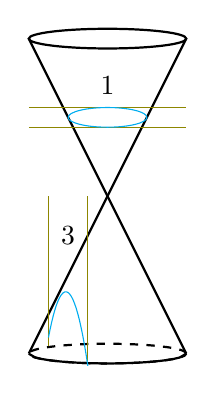
\begin{tikzpicture}[xscale=0.5,yscale=0.5]
    \draw[thick, domain=-2:2] plot (\x, {2*\x});
    \draw[thick, domain=-2:2] plot (\x, {-2*\x});
    \draw[thick] (0,4) ellipse (2 and 1/4);
    \draw[thick, domain=2:-2] plot (\x, {0.125*(-sqrt(4-(\x*\x))-32)});
    \draw[thick, dashed] (0,-4) ellipse (2 and 1/4);
    \draw[olive] (-2,1.75) -- (2,1.75);
    \draw[olive] (-2,2.25) -- (2,2.25);
    \draw[cyan] (0,2) ellipse (1 and 1/4);
    \node at (0,2.8) {1};
    \draw[olive] (-1.5,-3.8) -- (-1.5,0);
    \draw[olive] (-0.5,-4.2) -- (-0.5,0);
    \draw[cyan, domain=-1.5:-0.5] plot (\x, {-6*((\x+1.06)*(\x+1.06))-2.43});
    \node at (-1,-1) {3};
\end{tikzpicture} \hspace{50pt} 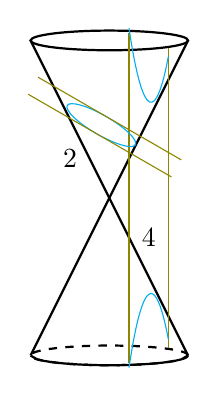
\begin{tikzpicture}[xscale=0.5,yscale=0.5]
    \draw[thick, domain=-2:2] plot (\x, {2*\x});
    \draw[thick, domain=-2:2] plot (\x, {-2*\x});
    \draw[thick] (0,4) ellipse (2 and 1/4);
    \draw[thick, domain=2:-2] plot (\x, {0.125*(-sqrt(4-(\x*\x))-32)});
    \draw[thick, dashed] (0,-4) ellipse (2 and 1/4);
    \draw[olive] (1.5,-3.8) -- (1.5,3.8);
    \draw[olive] (0.5,-4.2) -- (0.5,4.2);
    \draw[cyan, domain=1.5:0.5] plot (\x, {-6*((\x-1.06)*(\x-1.06))-2.43});
    \draw[cyan, domain=1.5:0.5] plot (\x, {6*((\x-1.06)*(\x-1.06))+2.43});
    \node at (1,-1) {4};
    \draw[cyan, rotate=330] (-1.1,1.5) ellipse (1 and 1/4);
    \draw[olive, rotate=330] (-3.1,1.75) -- (1.1,1.75);
    \draw[olive, rotate=330] (-3.1,1.25) -- (1.1,1.25);
    \node at (-1,1) {2};
\end{tikzpicture}
\end{center}

\begin{center}
\begin{tabular}{cccc}
1. Circle & 2. Ellipse & 3. Parabola & 4. Hyperbola \\
\end{tabular}
\end{center}

All conic sections can be described in terms of loci; for any point $P$ on a
conic section,

\[\frac{|PM|}{|PS|} = e\]

\noindent where $e$ is the eccentricity, $S$ is the focus and $M$ is the closest point to
$P$ that lies on the directrix.

\[0 \leq e < 1 \Rightarrow P \textrm{ describes an ellipse}\]
\[e = 1 \Rightarrow P \textrm{ describes a parabola}\]
\[e > 1 \Rightarrow P \textrm{ describes a hyperbola}\]

\begin{multicols}{2}

\vspace{20pt}

\begin{center}

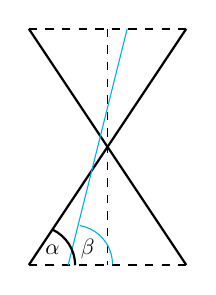
\begin{tikzpicture}[xscale=0.5,yscale=0.5]
    \draw[thick] (-2,-3) -- (2,3);
    \draw[thick] (-2,3) -- (2,-3);
    \draw[thick, dashed] (-2,-3) -- (2,-3);
    \draw[thick, dashed] (-2,3) -- (2,3);
    \draw[dashed] (0,3) -- (0,-3);
    \draw[cyan] (-1,-3) -- (0.5,3);
    \draw[cyan] (-0.7,-2) arc (80:0:1);
    \draw[thick] (-1.4,-2.1) arc (65:0:1);
    \node[scale=0.8] at (-1.4,-2.6) {\(\alpha\)};
    \node[scale=0.8] at (-0.5,-2.6) {\(\beta\)};
\end{tikzpicture}
\end{center}

\noindent The eccentricity can also be defined graphically, in terms of the cone and the intersection. Where \(e\) is the ratio between the angle of the cone and the intersection

\[e=\frac{\sin\left(\beta\right)}{\sin\left(\alpha\right)}\]

\end{multicols}


\subsection{Ellipses}

Ellipses are conic sections with eccentricty $e \in [0,1)$. Considering their
geometry, it is clear that, when expressed as a parametric equation, ellipses
take the form;

\[x = a\cos\theta,\: y = b\sin\theta\]

\noindent Hence;

\[\left(\frac{x}{a}\right)^2 = \cos^2\theta,\: \left(\frac{y}{b}\right)^2 =
\sin^2\theta\]

\noindent Making apparent an ellipse expressed in cartesian form;

\[\left(\frac{x}{a}\right)^2 + \left(\frac{y}{b}\right)^2 = 1\]

\paragraph{Theorem} For $e \in [0,1)$, an ellipse of focus $(ae, 0)$ and
directrix $x = \frac{a}{e}$ is described by the equation;

\[\left(\frac{x}{a}\right)^2 + \left(\frac{y}{b}\right)^2 = 1\]

\paragraph{Proof} 

\[\frac{|PS|^2}{|PM|^2} = e \Rightarrow |PS|^2 = e^2|PM|^2\]

\noindent By pythagoras,

\[|PS|^2 = \left(x - ae\right)^2 + y^2\]

\[|PM|^2 = \left(\frac{a}{e} - x\right)^2 + y^2\]

\noindent Thus

\[\left(x - ae\right)^2 + y^2 = \left(\frac{a}{e} - x\right)^2e^2\]\\

\noindent The derivative of an ellipse can be found by implicitly
differentiating its cartesian form or using the chain rule on its parametric
form. By the former method;

\[\frac{\de}{\de x} \left(\left(\frac{x}{a}\right)^2 +
\left(\frac{y}{b}\right)^2\right) = \frac{\de}{\de x}1\]

\[\frac{2x}{a^2} + \frac{2y}{b^2} \times \frac{\de y}{\de x} = 0\]

\[\frac{\de y}{\de x} = -\frac{b^2x}{a^2y}\]

\noindent And by the latter;

\[\frac{\de x}{\de \theta} = -a\sin\theta\]

\[\frac{\de y}{\de \theta} = b\cos\theta\]

\[\frac{\de y}{\de x} = \frac{\de y}{\de \theta} \times \left(\frac{\de x}{\de
\theta}\right)^{-1} = -\frac{b\cos\theta}{a\sin\theta}\]

\noindent From this we can derive the general equation of a tangent to an
ellipse at a point $\left(i,\, j\right)$:

\[y - j = -\frac{b^2i}{a^2j}\left(x - i\right)\]

\[a^2jy + b^2ix = \left(aj\right)^2 + \left(bi\right)^2\]

\noindent Similarly, we can derive the equation for a normal:

\[y - j = \frac{a^2j}{b^2i}\left(x - i\right)\]

\[b^2iy + a^2ij = a^2jx + b^2ij\]

\end{document}

